\documentclass{tietreport}

% Packages
\usepackage{graphicx}
\usepackage{amsmath}
\usepackage{booktabs}
\usepackage{array}
\usepackage{float}
\usepackage{tikz}
\usepackage{xcolor}
\usepackage{tabularx}
\usepackage{hyperref}

\usetikzlibrary{arrows.meta, positioning, shapes.geometric, shapes.misc}

% Soft pink formula highlighting
\definecolor{formulaPink}{RGB}{255,235,243}

% Numbered formula in a soft pink box; preserves equation numbering.
\newcommand{\pinkformula}[2][]{%
  \begin{equation}
    \begingroup
    \setlength{\fboxsep}{7pt}%
    \colorbox{formulaPink}{$\displaystyle #2$}%
    \endgroup
    \if\relax\detokenize{#1}\relax\else\label{#1}\fi
  \end{equation}
}

% Diagram styles
\tikzset{
  flowbox/.style={
    rectangle, rounded corners=3pt,
    draw=blue!55!black, fill=blue!5,
    line width=0.8pt, text width=2.25cm,
    minimum height=0.95cm, align=center, font=\small
  },
  flowdecision/.style={
    diamond, aspect=2.0,
    draw=orange!75!black, fill=orange!10,
    line width=0.8pt, text width=1.5cm,
    align=center, font=\small, inner sep=2pt
  },
  flowarrow/.style={
    -{Stealth[length=2mm]}, line width=0.8pt,
    draw=gray!75!black
  },
  lifecyclebox/.style={
    rectangle, rounded corners=4pt,
    draw=#1, fill=#1!8, line width=0.9pt,
    text width=2.15cm, minimum height=0.9cm,
    align=center, font=\small
  }
}

% Avoid unnecessary blank verso pages in classes using double-sided chapters.
\let\cleardoublepage\clearpage

% Bibliography configuration from the TIET template
\usepackage[
  date=year,
  style=alphabetic,
  backend=biber,
  sorting=nty,
  maxnames=5,
  minnames=3,
  maxalphanames=4,
  minalphanames=3,
  backref=true,
  doi=false,
  isbn=false,
  url=false,
  eprint=false
]{biblatex}
\addbibresource{references.bib}

% ==================================================
% TITLE PAGE: REPLACE THE PLACEHOLDERS
% ==================================================


\TitlePageHeader{UCS503 -- Software Engineering}


\ProjectTitle{UberLite}

\ProjectSubTitle{Design and Implementation of a Full-Stack
Ride-Sharing Management Prototype}


\author{%
  \texttt{1024030740} Ayush\\
  \texttt{1024030749} Anshika\\
  \texttt{1024030325} Gurleen Kaur%
}

\TitlePageSubText{%
  Group: 3C53, BE, Computer Engineering%
}

\AdvisorName{Dr. Paramveer Kaur}

\TitlePageFooterText{{%
  \large Mid-Semester Evaluation \\[0.2cm]
  \bfseries Computer Science and Engineering Department%
  } \\[0.15cm]
  Thapar Institute of Engineering and Technology, Patiala%
}

\begin{document}

% Prevent excessive vertical whitespace on pages with figures and short sections.
\raggedbottom

\maketitle
\tableofcontents

% ==================================================
% CHAPTER 1: INTRODUCTION
% ==================================================

\chapter{Introduction}

\section{Background and Context}

Ride-sharing applications provide a digital platform through which
passengers can request transportation and drivers can accept and
complete trips. Such applications require coordination between
passengers, drivers, location information, ride status, and fare
calculation.

A ride-sharing system must handle several connected operations,
including user authentication, driver availability, assignment of
drivers to ride requests, tracking of ride progress, and maintaining
ride records. These operations must be coordinated to provide a
consistent experience for both passengers and drivers.

UberLite is a full-stack ride-sharing management prototype developed
to demonstrate these core operations. The system provides separate
passenger and driver interfaces supported by a backend API and a
relational database. It incorporates location-based driver matching,
distance-based fare estimation, controlled ride-state transitions,
and post-ride feedback.

The current implementation focuses on establishing a complete and
testable ride-booking workflow. More advanced capabilities, including
WebSocket-based updates and optimized spatial searching, are
identified as future enhancements.

\subsection{Problem Statement}

A ride-sharing application must coordinate ride requests with
available drivers while maintaining consistent ride status and driver
availability. A poorly coordinated system may assign conflicting
requests to the same driver, permit invalid ride-state transitions,
or calculate fares inconsistently.

The problem addressed by UberLite is the design and implementation
of a modular ride-sharing prototype that connects passenger requests,
driver assignment, ride execution, fare calculation, and feedback
within a unified full-stack application.

The system must enforce role-based access, validate incoming
requests, preserve consistent ride-state transitions, and store
relevant information in a relational database. It should also provide
a foundation for future improvements in real-time communication,
matching efficiency, and scalability.

\section{Project Objectives}

The project has the following objectives:

\begin{enumerate}
    \item \textbf{Authentication and authorization:}
    Implement registration and login for passengers and drivers,
    with JWT-based authentication and role-based access control.

    \item \textbf{Location-based driver matching:}
    Develop a location utility using the Haversine formula and
    assign the nearest eligible available driver to a ride request.

    \item \textbf{Ride lifecycle management:}
    Implement the ride workflow from request through acceptance
    and initiation to completion, while rejecting invalid
    state transitions.

    \item \textbf{Fare calculation:}
    Implement fare estimation based on a base fare and the
    calculated travel distance, with final fare calculation
    upon ride completion.

    \item \textbf{Full-stack integration:}
    Connect the passenger and driver dashboards to backend APIs
    and persist application data using PostgreSQL and Prisma ORM.

    \item \textbf{Testing and verification:}
    Validate core functionality through unit and integration
    tests and verify that the application builds successfully.
\end{enumerate}

The objectives are intended to be achieved incrementally, with
the initial phase prioritizing a working end-to-end ride-booking
workflow before advanced optimization and real-time features.

% ==================================================
% CHAPTER 2: METHODOLOGY AND DESIGN
% ==================================================

\chapter{Methodology and Design}

\section{System Architecture}

UberLite follows a modular full-stack architecture. The frontend
provides user interfaces for passengers and drivers, while the
backend exposes APIs for authentication, driver management,
ride operations, fare calculation, and feedback.

The backend communicates with a PostgreSQL database through
Prisma ORM. Request validation and authentication middleware
are used to validate incoming data and restrict access to
role-specific operations.

\subsection{High-Level Design}

The system consists of the following major components:

\begin{enumerate}
    \item \textbf{Frontend layer:}
    The React application provides registration and login,
    passenger and driver dashboards, ride-request controls,
    ride-status information, history, and feedback interfaces.

    \item \textbf{API and middleware layer:}
    The Express backend handles HTTP requests, authentication,
    role-based authorization, request validation, and error
    responses.

    \item \textbf{Service layer:}
    Modular services implement location calculations, driver
    matching, ride-state transitions, fare calculation,
    and other business operations.

    \item \textbf{Data layer:}
    PostgreSQL stores application records, while Prisma ORM
    provides database access, schema management, and
    transaction support.

    \item \textbf{Testing and deployment layer:}
    Automated tests verify application behaviour, and
    Docker and deployment configurations support preparation
    for demonstration and deployment.
\end{enumerate}

The principal request flow is:

\begin{figure}[H]
\centering
\resizebox{\textwidth}{!}{%
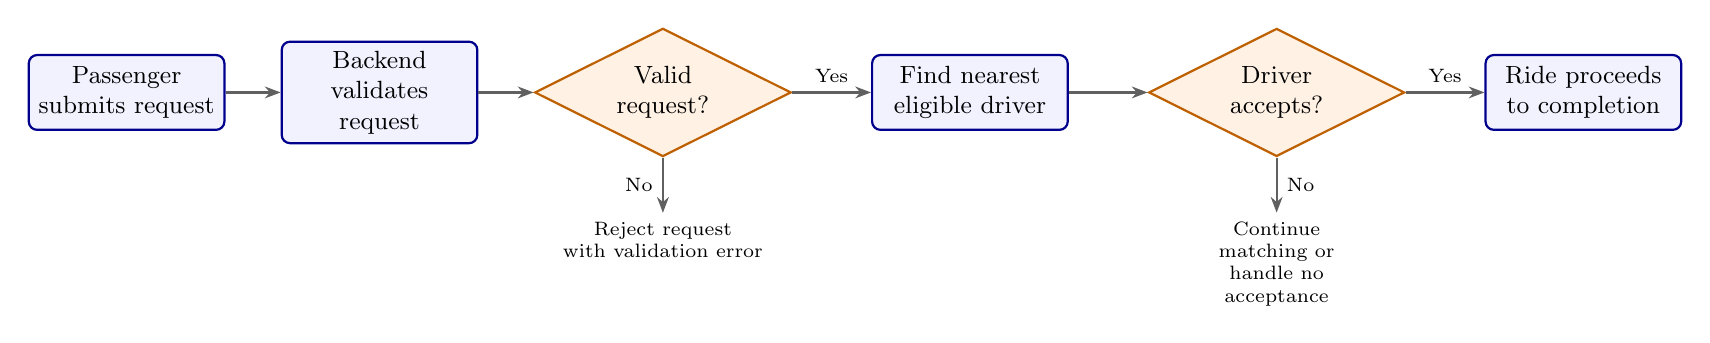
\begin{tikzpicture}[node distance=0.55cm and 0.7cm]
\node[flowbox] (passenger) {Passenger\\submits request};
\node[flowbox, right=of passenger] (validate) {Backend validates\\request};
\node[flowdecision, right=of validate] (valid) {Valid\\request?};
\node[flowbox, right=1.0cm of valid] (match) {Find nearest\\eligible driver};
\node[flowdecision, right=1.0cm of match] (driver) {Driver\\accepts?};
\node[flowbox, right=1.0cm of driver] (ride) {Ride proceeds\\to completion};

\draw[flowarrow] (passenger.east) -- (validate.west);
\draw[flowarrow] (validate.east) -- (valid.west);
\draw[flowarrow] (valid.east) --
  node[above, font=\scriptsize] {Yes} (match.west);
\draw[flowarrow] (match.east) -- (driver.west);
\draw[flowarrow] (driver.east) --
  node[above, font=\scriptsize] {Yes} (ride.west);

\node[below=0.7cm of valid, font=\scriptsize, align=center,
  text width=2.6cm] (invalid) {Reject request\\with validation error};
\draw[flowarrow] (valid.south) --
  node[left, font=\scriptsize] {No} (invalid.north);

\node[below=0.7cm of driver, font=\scriptsize, align=center,
  text width=2.6cm] (retry) {Continue matching or\\handle no acceptance};
\draw[flowarrow] (driver.south) --
  node[right, font=\scriptsize] {No} (retry.north);
\end{tikzpicture}%
}
\caption{Principal request flow in UberLite}
\label{fig:request-flow}
\end{figure}

Responses travel back through the backend API to the relevant
frontend interface. The current dashboard implementation uses
HTTP polling for ride-status updates rather than a WebSocket
connection.

\subsection{Technical Stack}

The technologies used in the reported implementation are
summarized in Table~\ref{tab:techstack}.

\begin{table}[H]
\centering
\small
\renewcommand{\arraystretch}{1.25}
\begin{tabularx}{\textwidth}{p{0.22\textwidth} p{0.27\textwidth} X}
\toprule
\textbf{Component} & \textbf{Technology} & \textbf{Purpose} \\
\midrule
Frontend & React 19, TypeScript, Vite & Provides passenger and driver interfaces. \\
Backend & Node.js, Express & Handles API requests and business logic. \\
Database & PostgreSQL & Stores persistent application and ride data. \\
ORM & Prisma ORM & Provides structured database access. \\
Request validation & Zod & Validates incoming request data. \\
Authentication & JSON Web Tokens (JWT) & Supports token-based authentication. \\
Location calculation & Haversine formula & Estimates distance between coordinates. \\
Testing & Unit and integration tests & Checks core application behaviour. \\
Infrastructure & Docker, Docker Compose & Supports containerization and deployment preparation. \\
\bottomrule
\end{tabularx}
\caption{Technology stack and component responsibilities}
\label{tab:techstack}
\end{table}

\section{Implementation Details}

The implementation was organized into modular components so
that the core ride-booking workflow could be developed and
tested incrementally.

\subsection{Module 1: Core Functionality}

\subsubsection*{Authentication and Authorization}

The authentication module supports registration and login
for passengers and drivers. Incoming requests are validated,
and authenticated sessions use JSON Web Tokens. Role-based
middleware restricts protected operations to the appropriate
user role.

Frontend route guards provide corresponding protection for
passenger and driver application areas. Figure~\ref{fig:signin-screen}
shows the sign-in interface, while Figure~\ref{fig:registration-screens}
shows the role-specific registration forms for passengers and drivers.

\begin{figure}[H]
\centering
\includegraphics[width=0.38\textwidth]{screenshots/signin.png}
\caption{UberLite sign-in interface with passenger and driver demo-account options.}
\label{fig:signin-screen}
\end{figure}

\begin{figure}[H]
\centering
\begin{minipage}[t]{0.34\textwidth}
  \centering
  \includegraphics[width=\linewidth]{screenshots/register_passenger.png}
  \par\smallskip
  {\small (a) Passenger registration}
\end{minipage}\hfill
\begin{minipage}[t]{0.34\textwidth}
  \centering
  \includegraphics[width=\linewidth]{screenshots/register_driver.png}
  \par\smallskip
  {\small (b) Driver registration}
\end{minipage}
\caption{Role-specific registration forms in UberLite. The driver form additionally collects vehicle and driving-licence information.}
\label{fig:registration-screens}
\end{figure}

\subsubsection*{Location Calculation and Driver Matching}

The location utility calculates the distance between two
geographic coordinates using the Haversine formula
\cite{haversine}. For coordinates represented by latitude
$\phi$ and longitude $\lambda$, the calculation uses:

\begin{samepage}
\pinkformula{%
a = \sin^2\left(\frac{\Delta\phi}{2}\right)
+ \cos(\phi_1)\cos(\phi_2)
  \sin^2\left(\frac{\Delta\lambda}{2}\right)
}

\pinkformula{d = 2R\arcsin\left(\sqrt{a}\right)}

where $R$ is the assumed Earth radius, the angles are
expressed in radians, and $d$ is the calculated great-circle
distance.
\end{samepage}

The matching service considers available drivers, calculates
their distance from the passenger's pickup location, and
selects the nearest eligible driver. The initial matching
approach uses a linear search. Transaction-safe assignment
logic is used to reduce the risk of assigning the same driver
to conflicting ride requests.

\subsubsection*{Ride Lifecycle Management}

A ride progresses through the following states:

\begin{figure}[htbp]
\centering
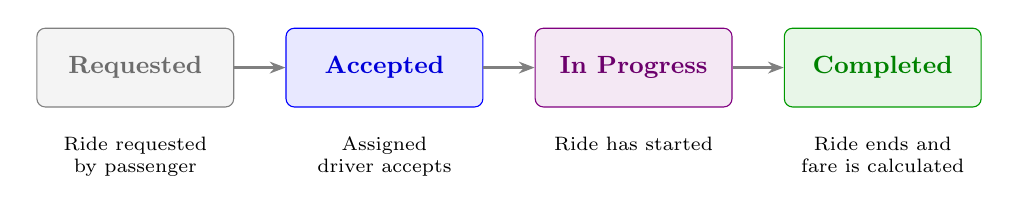
\begin{tikzpicture}[
    state/.style={
        rectangle,
        rounded corners=3pt,
        draw=#1,
        fill=#1!9,
        text=#1!85!black,
        minimum width=2.5cm,
        minimum height=1cm,
        align=center,
        font=\small\bfseries
    },
    flow/.style={
        -{Stealth[length=2mm]},
        thick,
        gray
    }
]
\node[state=gray] (requested) {Requested};
\node[state=blue, right=0.65cm of requested] (accepted) {Accepted};
\node[state=violet, right=0.65cm of accepted] (progress) {In Progress};
\node[state=green!60!black, right=0.65cm of progress] (completed) {Completed};

\draw[flow] (requested) -- (accepted);
\draw[flow] (accepted) -- (progress);
\draw[flow] (progress) -- (completed);

\node[below=0.25cm of requested, font=\scriptsize,
    text width=2.5cm, align=center]
    {Ride requested by passenger};

\node[below=0.25cm of accepted, font=\scriptsize,
    text width=2.5cm, align=center]
    {Assigned driver accepts};

\node[below=0.25cm of progress, font=\scriptsize,
    text width=2.5cm, align=center]
    {Ride has started};

\node[below=0.25cm of completed, font=\scriptsize,
    text width=2.5cm, align=center]
    {Ride ends and fare is calculated};
\end{tikzpicture}
\caption{Ride lifecycle and valid state transitions in UberLite.}
\label{fig:ride-lifecycle}
\end{figure}

The backend validates state transitions and rejects invalid
operations, such as completing a ride that has not started.
Driver availability is updated as the ride starts and
finishes, helping prevent conflicting assignments.

\subsubsection*{Fare Calculation}

The fare module estimates the cost of a ride using a base
fare and a distance-based rate. The fare model is:

\pinkformula[eq:fare]{F = B + (D \times r)}

where $F$ represents the fare, $B$ is the base fare,
$D$ is the distance used for fare calculation, and $r$
is the rate per unit distance.

The final fare is calculated when the ride is completed
and persisted with the ride record. The configured fare
parameters are maintained by the application.

\subsection{Module 2: Secondary Features}

\subsubsection*{Passenger and Driver Dashboards}

The passenger dashboard supports ride requests, estimated
fare information, ride-status updates, driver information,
and post-ride feedback. The driver dashboard supports
availability controls, incoming ride requests, and actions
for accepting and progressing assigned rides.

The dashboards communicate with the backend through HTTP
APIs. Polling is used to refresh relevant ride information.
Figure~\ref{fig:passenger-dashboard-screens} illustrates the
ride-request view, including pickup and drop-off locations and fare
estimation, alongside the active-ride view with progress status and
assigned-driver information.

\begin{figure}[htbp]
\centering
\begin{minipage}[t]{0.49\textwidth}
  \centering
  \includegraphics[width=\linewidth]{screenshots/passenger_book_ride.png}
  \par\smallskip
  {\small (a) Ride request and fare estimate}
\end{minipage}\hfill
\begin{minipage}[t]{0.43\textwidth}
  \centering
  \includegraphics[width=\linewidth]{screenshots/passenger_active_ride.png}
  \par\smallskip
  {\small (b) Active ride and assigned driver}
\end{minipage}
\caption{Passenger dashboard views in UberLite.}
\label{fig:passenger-dashboard-screens}
\end{figure}

\subsubsection*{Ride History and Feedback}

The application includes ride-history APIs and corresponding
history interfaces for passengers and drivers. Relevant
information includes ride details, status, fare, and
completion information.

After a ride has been completed, the passenger can submit
a rating and optional feedback associated with the ride
and its driver.

\subsubsection*{Validation and Error Handling}

Zod is used for request validation, while centralized
backend error handling provides consistent responses for
invalid input, unauthorized operations, missing resources,
and invalid workflow transitions.

Database relationships, constraints, and transaction handling
support data consistency across related operations.

\subsubsection*{Integration and Deployment Preparation}

The frontend and backend have been integrated to support
the main ride-booking workflow. The project also contains
Dockerfiles, Docker Compose orchestration, and configurations
for deployment platforms.

These configurations provide deployment preparation; they
should not be interpreted as evidence of a publicly deployed
production service.

% ==================================================
% CHAPTER 3: RESULTS AND EVALUATION
% ==================================================

\chapter{Results and Evaluation}

\section{Testing Methodology}

Testing was carried out to verify the correctness of the
individual modules and their interaction across the
full-stack application.

\begin{itemize}
    \item \textbf{Unit testing:}
    Tests cover individual operations, including location
    calculations, fare calculation, matching logic, ride-state
    transitions, and validation rules.

    \item \textbf{Integration testing:}
    Tests cover connected workflows such as registration,
    login, role-based access, ride creation, driver matching,
    ride progression, fare persistence, history, and feedback.

    \item \textbf{Frontend testing:}
    Tests validate session storage, protected routes,
    form validation, and authentication-related UI states.

    \item \textbf{Build verification:}
    Production TypeScript compilation and application builds
    are used to identify compilation and build errors.

    \item \textbf{Performance evaluation:}
    Backend instrumentation records relevant timing and
    workflow information. A separate load-testing study
    remains part of the future scope unless supported by
    additional measured results.
\end{itemize}

\section{Performance Metrics}

The current evaluation emphasizes automated test results
and build verification. Table~\ref{tab:testresults}
summarizes the results reported for the current prototype.

\begin{table}[H]
\centering
\small
\renewcommand{\arraystretch}{1.3}
\begin{tabularx}{0.92\textwidth}{X p{0.25\textwidth} p{0.18\textwidth}}
\toprule
\textbf{Metric} & \textbf{Reported result} & \textbf{Status} \\
\midrule
Backend automated tests & 307 passing & Reported pass \\
Frontend automated tests & 34 passing & Reported pass \\
Total passing tests & 341 & Reported pass \\
Production TypeScript build & Zero compilation errors & Reported pass \\
\bottomrule
\end{tabularx}
\caption{Reported testing and build results}
\label{tab:testresults}
\end{table}

The reported test results indicate that the prototype has
undergone automated verification across backend functionality
and frontend behaviour. The combined test count is 341,
based on the reported backend and frontend suite totals.

These results establish evidence of functional verification,
but do not by themselves establish production-scale throughput,
average response time, or real-world matching accuracy.
Those metrics require dedicated measurement under defined
test conditions.

\section{Technical Development Progress}

The technical development is organized into the core application workflow
followed by verification and planned engineering improvements. The first
stages establish the database and backend, authentication, ride management,
and frontend integration. Testing and validation are used to verify the
implemented functionality. Real-time communication and performance
optimization remain planned improvements.

\begin{figure}[htbp]
\centering
\resizebox{\textwidth}{!}{%
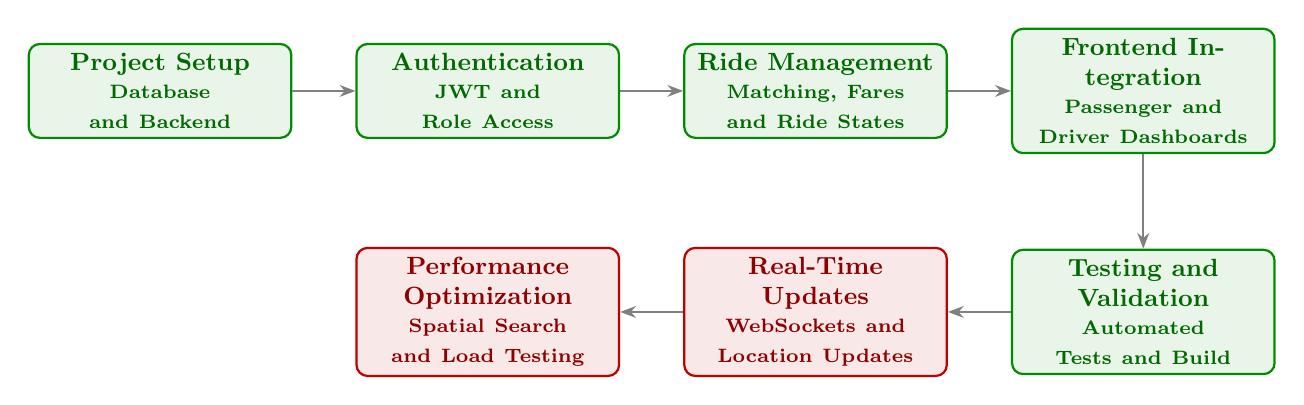
\begin{tikzpicture}[
    node distance=0.55cm and 0.8cm,
    stage/.style={
        rectangle,
        rounded corners=4pt,
        draw=#1,
        fill=#1!9,
        text=#1!75!black,
        line width=0.8pt,
        text width=3.1cm,
        minimum height=0.9cm,
        align=center,
        font=\small\bfseries
    },
    flow/.style={
        -{Stealth[length=2mm]},
        thick,
        gray
    }
]
% Green boxes: core work completed, including reported testing/build checks
\node[stage=green!55!black] (setup)
    {Project Setup\\[-1pt]\scriptsize Database and Backend};
\node[stage=green!55!black, right=of setup] (auth)
    {Authentication\\[-1pt]\scriptsize JWT and Role Access};
\node[stage=green!55!black, right=of auth] (core)
    {Ride Management\\[-1pt]\scriptsize Matching, Fares and Ride States};
\node[stage=green!55!black, right=of core] (frontend)
    {Frontend Integration\\[-1pt]\scriptsize Passenger and Driver Dashboards};
\node[stage=green!55!black, below=1.2cm of frontend] (testing)
    {Testing and Validation\\[-1pt]\scriptsize Automated Tests and Build};
% Red boxes: pending technical improvements
\node[stage=red!75!black, left=of testing] (realtime)
    {Real-Time Updates\\[-1pt]\scriptsize WebSockets and Location Updates};
\node[stage=red!75!black, left=of realtime] (optimization)
    {Performance Optimization\\[-1pt]\scriptsize Spatial Search and Load Testing};
\draw[flow] (setup) -- (auth);
\draw[flow] (auth) -- (core);
\draw[flow] (core) -- (frontend);
\draw[flow] (frontend.south) -- ++(0,-0.45) -| (testing.north);
\draw[flow] (testing.west) -- (realtime.east);
\draw[flow] (realtime.west) -- (optimization.east);
\end{tikzpicture}%
}
\caption{Technical development progress and planned improvements in UberLite}
\label{fig:technical-progress}
\end{figure}

\section{Analysis}

The current implementation addresses the principal objectives
of the project by providing an integrated ride-booking
workflow. Authentication and authorization separate passenger
and driver operations, while backend validation restricts
invalid requests and ride-state transitions.

The location-based matching service provides a functional
baseline for assigning available drivers. However, its
linear search approach may become less efficient as the
number of available drivers increases. Spatial indexing or
bounding-box-based filtering can be investigated in a
subsequent phase.

The current polling mechanism supports ride-status
synchronization but introduces repeated HTTP requests.
WebSocket-based communication could reduce unnecessary
polling and provide more immediate updates.

The implementation also includes transaction-safe driver
assignment to improve consistency during concurrent requests.
Further concurrency and load testing is needed to quantify
its behaviour under heavier workloads.

Overall, the prototype provides a foundation for evaluating
the core ride-booking workflow. Additional performance
measurements, broader user evaluation, and deployment testing
would strengthen the assessment beyond functional correctness.

% ==================================================
% CHAPTER 4: CONCLUSION
% ==================================================

\chapter{Conclusion}

\section{Summary of Work}

UberLite has progressed from initial project setup to an
integrated full-stack ride-sharing prototype. The reported
implementation includes a React and TypeScript frontend,
an Express backend, and a PostgreSQL database managed
through Prisma ORM.

The completed core workflow covers passenger and driver
authentication, role-based authorization, location-based
driver matching, ride-state transitions, fare calculation,
dashboards, ride history, and feedback.

Automated backend and frontend tests have been reported
as passing, and production build verification has been
reported as successful. These results provide an initial
basis for evaluating the correctness of the implemented
functionality.

\section{Key Findings}

The current implementation supports the following findings:

\begin{itemize}
    \item A modular full-stack architecture can connect
    authentication, driver matching, ride management,
    and fare calculation into one workflow.

    \item Backend validation, role-based authorization,
    and controlled ride-state transitions help enforce
    application rules and restrict invalid operations.

    \item Automated tests provide evidence of functional
    correctness, while further performance testing is
    required to evaluate scalability and response times
    under heavier workloads.
\end{itemize}

\section{Future Work and Recommendations}

The next phase will focus on improving the efficiency,
responsiveness, and scalability of the prototype.

\begin{enumerate}
    \item \textbf{Driver search optimization:}
    Replace or optimize the initial linear driver search
    using spatial indexing or bounding-box-based queries.

    \item \textbf{Real-time communication:}
    Introduce WebSockets for passenger and driver ride-status
    synchronization while retaining the REST API as the
    source of ride state.

    \item \textbf{Driver location updates:}
    Implement periodic location updates to improve the
    freshness of driver coordinates used for matching
    and future ride tracking.

    \item \textbf{Concurrency and history improvements:}
    Extend concurrent ride-request testing and add practical
    filtering to ride-history interfaces.

    \item \textbf{Frontend improvements:}
    Improve responsiveness, usability, loading states,
    and error presentation across different screen sizes.

    \item \textbf{Performance and scalability evaluation:}
    Measure API response times, driver-assignment latency,
    and system behaviour under increasing numbers of
    drivers and concurrent ride requests.

    \item \textbf{Deployment and documentation:}
    Verify the deployment workflow and prepare supporting
    architecture diagrams, API documentation, and
    demonstration instructions.
\end{enumerate}

\section{Final Remarks}

The current phase establishes the functional foundation
of UberLite as a full-stack ride-sharing management prototype.
It demonstrates the integration of frontend interfaces,
backend services, database persistence, driver matching,
and ride lifecycle management.

The subsequent development phase will build on this foundation
by improving real-time communication, search efficiency,
interface responsiveness, and performance evaluation.
These enhancements will help determine how effectively
the prototype can be extended beyond its current core
functionality.

% ==================================================
% BIBLIOGRAPHY
% ==================================================

\printbibliography[heading=bibintoc]

\end{document}